\chapter{Results}

\label{ch:Results}

In this chapter we will perform a number of experiments to assess the proposed methods from last chapter. We wish to keep the architectures fixed and vary the method, which is done to accurately assess its feasibility. Of course, some methods require a change in architecture, in which case we make the smallest possible change. First we will mention the architectures used, after which we will explore each proposed method in detail.

Unless specified otherwise, the Adam optimiser was used with a learning rate of $1e-3$. We also use a data set of $100,000$ pre-processed frames of Space Invaders (generated with the Arcade Learning Environment), with a $90$-$10$ training-test split. With such a large data set of high-dimensional data, we train the models with early stopping (until the gains are no longer qualitatively different) to ensure a breadth of parameters are explored.

%
%
%
%
%
\section{Architectures}

In this section we will use architectures similar to one proven to capture the generative factors in the Atari game \textit{Space Invaders} \cite{Higgins2016}. We do not claim that these architectures are optimal, but simply that they are capable of learning the generative factors in the scene.

The architectures used are specified in Tables (\ref{tab:fully_convolutional_single_filter}), (\ref{tab:fully_convolutional_multiple_filter}) and (\ref{tab:fully_convolutional_multiple_filter_rgb}).


\begin{table}[]
\centering
\begin{tabular}{@{}lll@{}}
\toprule
\textbf{Layer} & \textbf{Output shape} & \textbf{Connected to}  \\ \midrule
InputLayer     & (1, 84, 84)           &                        \\
Conv2D\_1      & (32, 42, 42)          & InputLayer             \\
Conv2D\_2      & (64, 21, 21)          & Conv2D\_1              \\
Conv2D\_3      & (1, 8, 8)             & Conv2D\_2              \\
Conv2D\_4      & (1, 8, 8)             & Conv2D\_2              \\
Sampling       & (1, 8, 8)             & Conv2D\_3 \& Conv2D\_4 \\
Deconv2D\_1    & (64, 20, 20)          & Sampling               \\
Deconv2D\_2    & (32, 40, 40)          & Deconv2D\_1            \\
Deconv2D\_3    & (1, 84, 84)           & Deconv2D\_2           
\end{tabular}
\caption{Fully-convolutional single-filter variational autoencoder.}
\label{tab:fully_convolutional_single_filter}
\end{table}


\begin{table}[]
\centering
\begin{tabular}{@{}lll@{}}
\toprule
\textbf{Layer} & \textbf{Output shape} & \textbf{Connected to}  \\ \midrule
InputLayer     & (1, 84, 84)           &                        \\
Conv2D\_1      & (32, 42, 42)          & InputLayer             \\
Conv2D\_2      & (64, 21, 21)          & Conv2D\_1              \\
Conv2D\_3      & (8, 8, 8)             & Conv2D\_2              \\
Conv2D\_4      & (8, 8, 8)             & Conv2D\_2              \\
Sampling       & (8, 8, 8)             & Conv2D\_3 \& Conv2D\_4 \\
Deconv2D\_1    & (64, 20, 20)          & Sampling               \\
Deconv2D\_2    & (32, 40, 40)          & Deconv2D\_1            \\
Deconv2D\_3    & (1, 84, 84)           & Deconv2D\_2           
\end{tabular}
\caption{Fully-convolutional multiple latent filter variational autoencoder.}
\label{tab:fully_convolutional_multiple_filter}
\end{table}


\begin{table}[]
\centering
\begin{tabular}{@{}lll@{}}
\toprule
\textbf{Layer} & \textbf{Output shape} & \textbf{Connected to}  \\ \midrule
InputLayer     & (3, 84, 84)           &                        \\
Conv2D\_1      & (32, 42, 42)          & InputLayer             \\
Conv2D\_2      & (64, 21, 21)          & Conv2D\_1              \\
Conv2D\_3      & (8, 8, 8)             & Conv2D\_2              \\
Conv2D\_4      & (8, 8, 8)             & Conv2D\_2              \\
Sampling       & (8, 8, 8)             & Conv2D\_3 \& Conv2D\_4 \\
Deconv2D\_1    & (64, 20, 20)          & Sampling               \\
Deconv2D\_2    & (32, 40, 40)          & Deconv2D\_1            \\
Deconv2D\_3    & (3, 84, 84)           & Deconv2D\_2           
\end{tabular}
\caption{Fully-convolutional multiple latent filter variational autoencoder for RGB images.}
\label{tab:fully_convolutional_multiple_filter_rgb}
\end{table}


%
%
%
%
%
\section{Single Latent Filter}

\subsection{Results}
The single latent architecture, found in Table (\ref{tab:fully_convolutional_single_filter}), was trained for $10$ epochs, and the validation, validation KL and validation reconstruction loss recorded. The results are shown in Figure (\ref{fig:latent_image_graphs}). The single latent image method is clearly capable of achieving reasonable reconstruction and KL loss on unseen data.

We see that the reconstructions of several inputs, shown in Figure (\ref{fig:latent_image_originals_and_reconstructions}), are qualitatively perfect. For each value of $\beta$, the reconstruction is indistinguishable from its input. This comes as quite a surprise, as we initially suspected this method is too restrained in the latent space.

The latent representations of scenes, shown in Figure (\ref{fig:latent_image_originals_and_latent_spaces}), do not meaningfully correspond to their original scene. Even for high $\beta$, the scenes do not seem to become anything more interpretable than noise. We further took the average of the latent filters over the test set of $10,000$ data points, and achieved similar results, which are shown in Figure (\ref{fig:latent_image_average_filters}).

Likewise, the decoded samples from the prior $p(\vec{z})$ and unknown distribution $\hat{p}(\vec{z})$, shown in Figures (\ref{fig:latent_image_originals_prior_samples}) and (\ref{fig:latent_image_originals_posterior_samples}) respectively, do not have any meaningful relation to the original scene. This is true for all values of $\beta$ tested. This tells us that even for reasonable values of the KL loss term, the latent image method struggles to generate realistic samples.

\subsection{Summary}
\begin{itemize}
\item The latent image method is capable of qualitatively perfect reconstruction of its input.
\item Despite the perfect reconstruction, the method seems to struggle with learning interpretable latent representations of high-level concepts in the scene for all values of $\beta$.
\item The latent image method also seemed to struggle to produce meaningful generative samples from the prior $p(\vec{z})$ and unknown distribution $\hat{p}(\vec{z})$ despite reasonable values of validation KL loss.
\end{itemize}


\begin{figure*}[h!]
\centering
\captionsetup{justification=centering}
    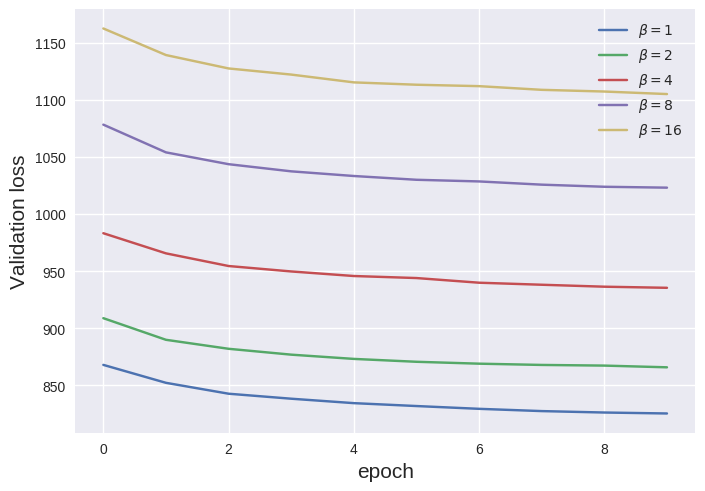
\includegraphics[scale=0.5]{figures/results/latent_image/val_loss.png}
    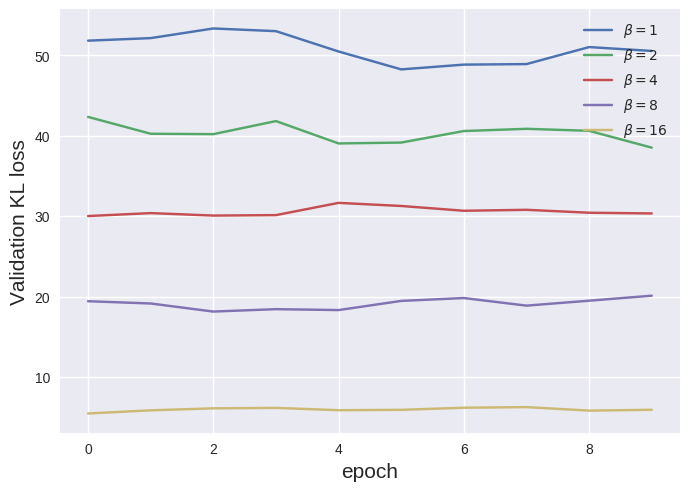
\includegraphics[scale=0.5]{figures/results/latent_image/val_kl_loss.png}
    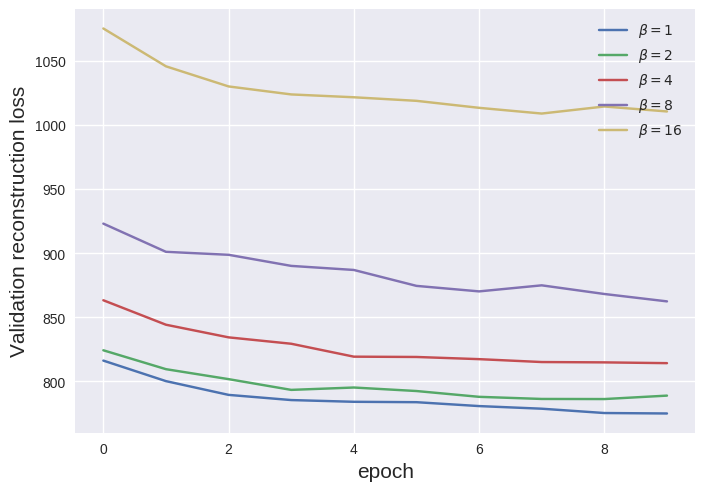
\includegraphics[scale=0.5]{figures/results/latent_image/val_reconstruction_loss.png}
\caption{\textbf{Single latent filter architecture}. The validation, validation KL and validation reconstruction loss for the latent image architecture and different values of $\beta$.}
\label{fig:latent_image_graphs}
\end{figure*}



\begin{figure*}[h!]
\centering
\captionsetup{justification=centering}
\begin{multicols}{4}
    \includegraphics[scale=0.4]{figures/results/latent_image/beta_1_sample_0_original.png}
    \caption{Original}
    \includegraphics[scale=0.4]{figures/results/latent_image/beta_1_sample_0_reconstructed.png}
    \caption{$\beta = 1$}    
    \includegraphics[scale=0.4]{figures/results/latent_image/beta_4_sample_0_reconstructed.png}
    \caption{$\beta = 4$}
    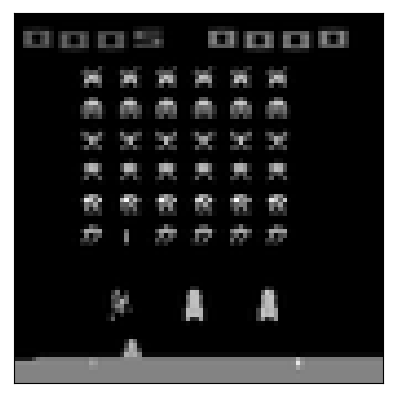
\includegraphics[scale=0.4]{figures/results/latent_image/beta_16_sample_0_reconstructed.png}
    \caption{$\beta = 16$}
\end{multicols}
\begin{multicols}{4}
    \includegraphics[scale=0.4]{figures/results/latent_image/beta_1_sample_2_original.png}
    \caption{Original}
    \includegraphics[scale=0.4]{figures/results/latent_image/beta_1_sample_2_reconstructed.png}
    \caption{$\beta = 1$}    
    \includegraphics[scale=0.4]{figures/results/latent_image/beta_4_sample_2_reconstructed.png}
    \caption{$\beta = 4$}
    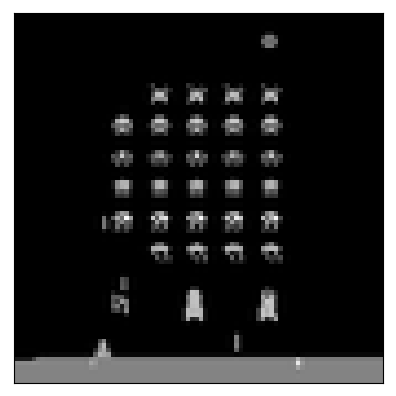
\includegraphics[scale=0.4]{figures/results/latent_image/beta_16_sample_2_reconstructed.png}
    \caption{$\beta = 16$}
\end{multicols}
\begin{multicols}{4}
    \includegraphics[scale=0.4]{figures/results/latent_image/beta_1_sample_3_original.png}
    \caption{Original}
    \includegraphics[scale=0.4]{figures/results/latent_image/beta_1_sample_3_reconstructed.png}
    \caption{$\beta = 1$}    
    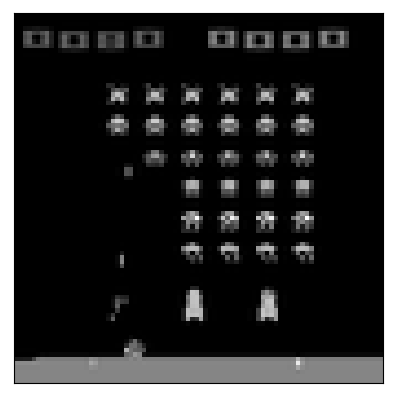
\includegraphics[scale=0.4]{figures/results/latent_image/beta_4_sample_3_reconstructed.png}
    \caption{$\beta = 4$}
    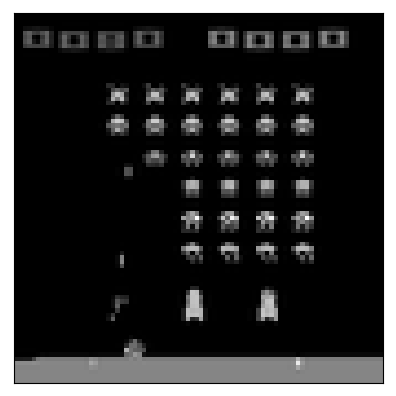
\includegraphics[scale=0.4]{figures/results/latent_image/beta_16_sample_3_reconstructed.png}
    \caption{$\beta = 16$}
\end{multicols}
\caption{\textbf{Single latent filter architecture}. A selection of Space Invader frames and their corresponding reconstructions for different values of $\beta$.}
\label{fig:latent_image_originals_and_reconstructions}
\end{figure*}


\begin{figure*}[h!]
\centering
\captionsetup{justification=centering}
\begin{multicols}{4}
    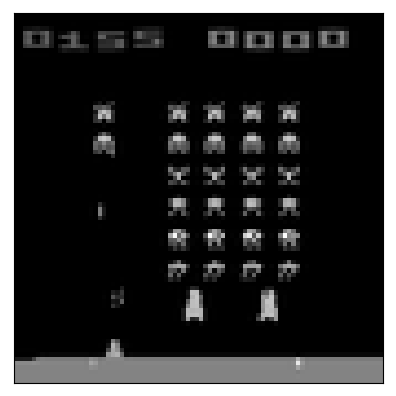
\includegraphics[scale=0.4]{figures/results/latent_image/beta_1_sample_10_original.png}
    \caption{Original}
    
\includegraphics[scale=0.4]{figures/results/latent_image/beta_1_sample_10_latent.png}
    \caption{$\beta=1$}
    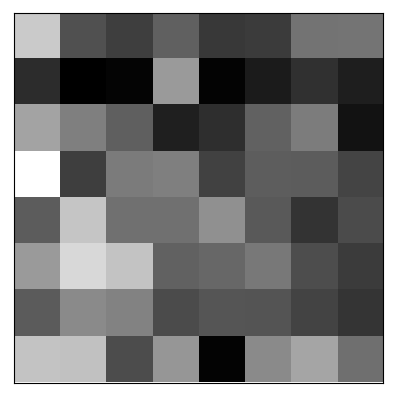
\includegraphics[scale=0.4]{figures/results/latent_image/beta_4_sample_10_latent.png}
    \caption{$\beta=4$}
    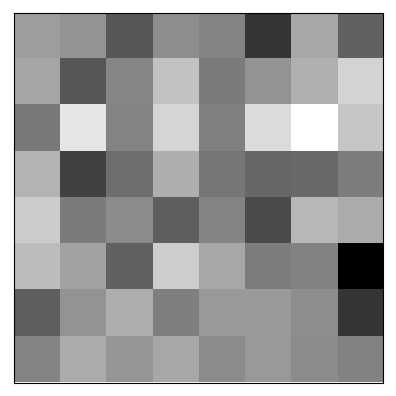
\includegraphics[scale=0.4]{figures/results/latent_image/beta_16_sample_10_latent.png}
    \caption{$\beta=16$}
\end{multicols}
\begin{multicols}{4}
    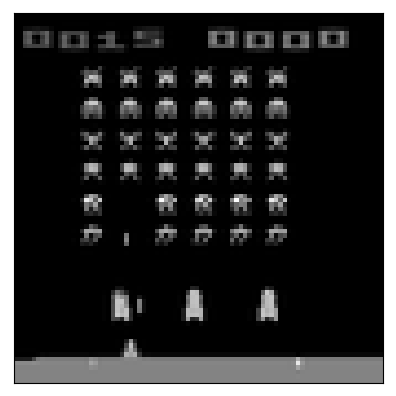
\includegraphics[scale=0.4]{figures/results/latent_image/beta_1_sample_30_original.png}
    \caption{Original}
    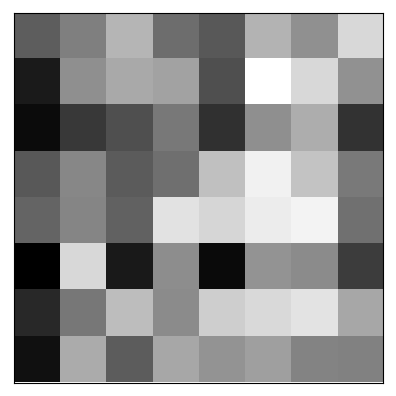
\includegraphics[scale=0.4]{figures/results/latent_image/beta_1_sample_30_latent.png}
    \caption{$\beta=1$}
    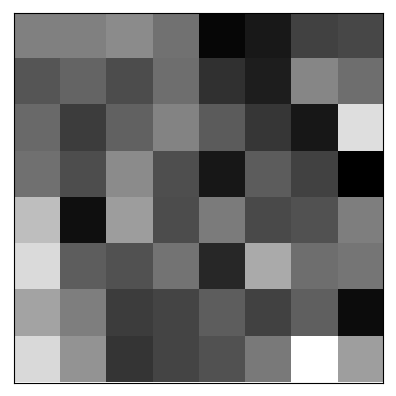
\includegraphics[scale=0.4]{figures/results/latent_image/beta_4_sample_30_latent.png}
    \caption{$\beta=4$}
    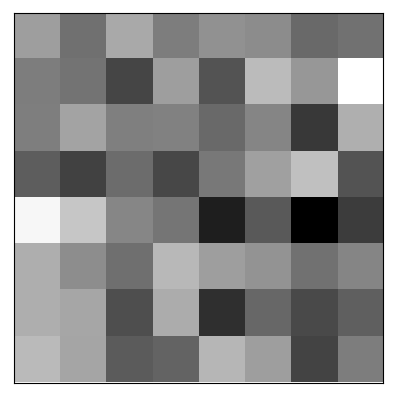
\includegraphics[scale=0.4]{figures/results/latent_image/beta_16_sample_30_latent.png}
    \caption{$\beta=16$}
\end{multicols}
\begin{multicols}{4}
    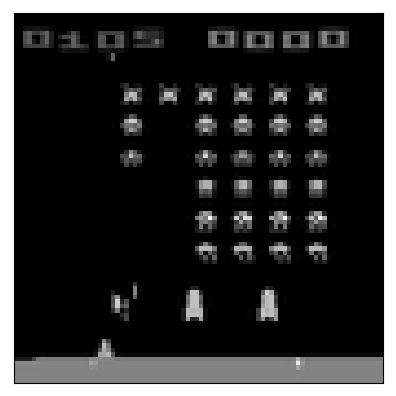
\includegraphics[scale=0.4]{figures/results/latent_image/beta_1_sample_90_original.png}
    \caption{Original}
    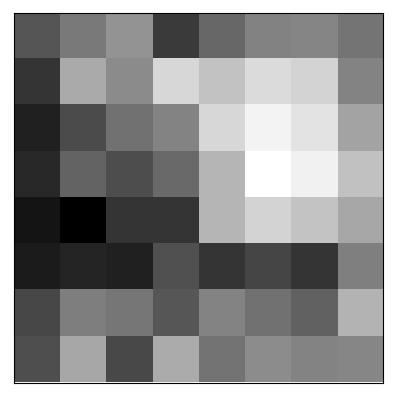
\includegraphics[scale=0.4]{figures/results/latent_image/beta_1_sample_90_latent.png}
    \caption{$\beta=1$}
    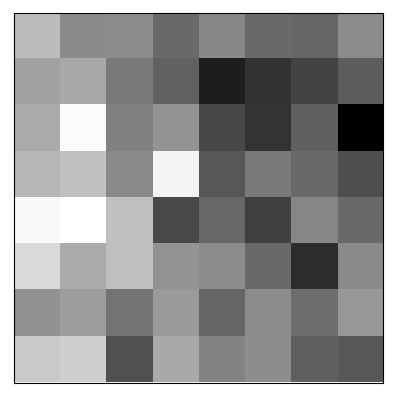
\includegraphics[scale=0.4]{figures/results/latent_image/beta_4_sample_90_latent.png}
    \caption{$\beta=4$}
    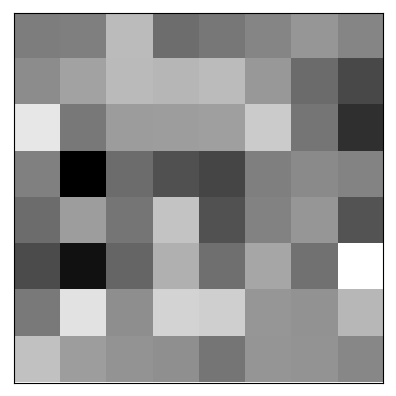
\includegraphics[scale=0.4]{figures/results/latent_image/beta_16_sample_90_latent.png}
    \caption{$\beta=16$}
\end{multicols}
\caption{\textbf{Single latent filter architecture}. Frames from Space Invaders and their corresponding latent images for different values of $\beta$.}
\label{fig:latent_image_originals_and_latent_spaces}
\end{figure*}


\begin{figure*}[h!]
\centering
\captionsetup{justification=centering}
\begin{multicols}{3}
    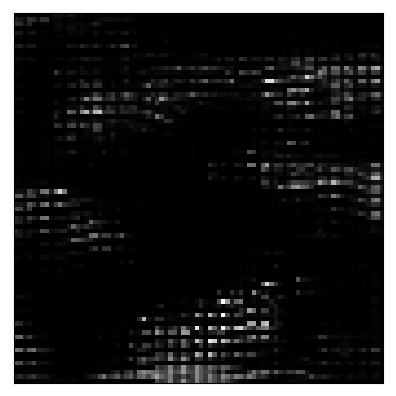
\includegraphics[scale=0.4]{figures/results/latent_image/beta_1_prior_sample_1.png}
    \caption{$\beta=1$}
    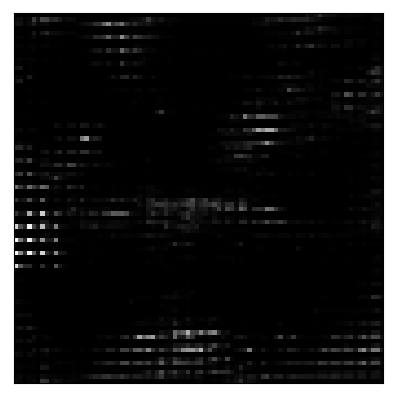
\includegraphics[scale=0.4]{figures/results/latent_image/beta_4_prior_sample_2.png}
    \caption{$\beta=4$}
    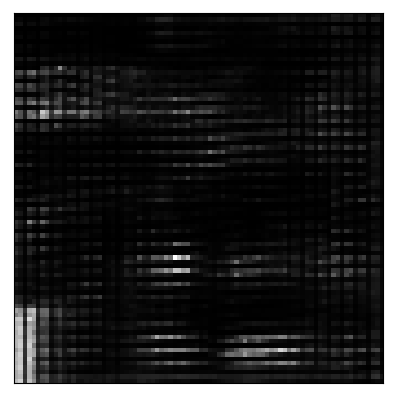
\includegraphics[scale=0.4]{figures/results/latent_image/beta_16_prior_sample_1.png}
    \caption{$\beta=16$}
\end{multicols}
\caption{\textbf{Single latent filter architecture}. The best of $10$ samples from the prior $p(\vec{z}) = \mathcal{N}(\vec{0}, \vec{I})$ for different values of $\beta$.}
\label{fig:latent_image_originals_prior_samples}
\end{figure*}


\begin{figure*}[h!]
\centering
\captionsetup{justification=centering}
\begin{multicols}{4}
    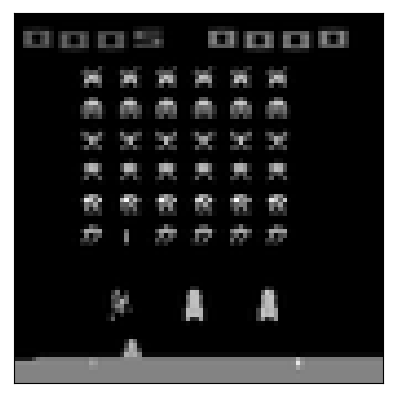
\includegraphics[scale=0.4]{figures/results/latent_image/beta_1_posterior_sample_original.png}
    \caption{Original}
    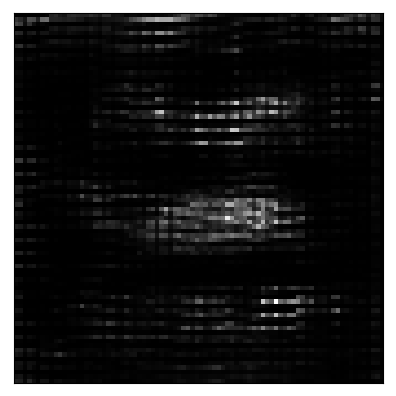
\includegraphics[scale=0.4]{figures/results/latent_image/beta_1_posterior_sample_0.png}
    \caption{$\beta=1$}
    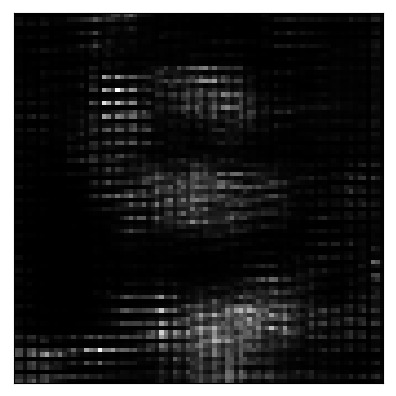
\includegraphics[scale=0.4]{figures/results/latent_image/beta_4_posterior_sample_0.png}
    \caption{$\beta=4$}
    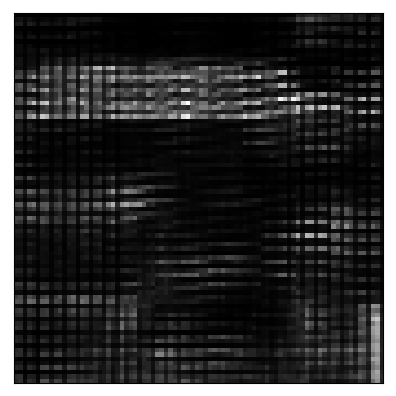
\includegraphics[scale=0.4]{figures/results/latent_image/beta_16_posterior_sample_11.png}
    \caption{$\beta=16$}
\end{multicols}
\caption{\textbf{Single latent filter architecture}. Samples from the unknown distribution $\hat{p}(\vec{z})$ after one step of MCMC for different values of $\beta$. Samples for subsequent steps did not improve, hence we only include the first for each value of $\beta$.}
\label{fig:latent_image_originals_posterior_samples}
\end{figure*}


\begin{figure*}[h!]
\centering
\captionsetup{justification=centering}
\begin{multicols}{3}
    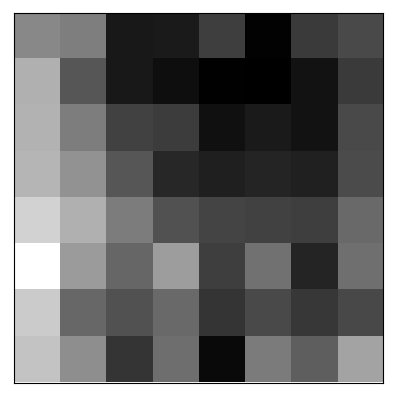
\includegraphics[scale=0.4]{figures/results/latent_image/beta_1_average_activation.png}
    \caption{$\beta=1$}
    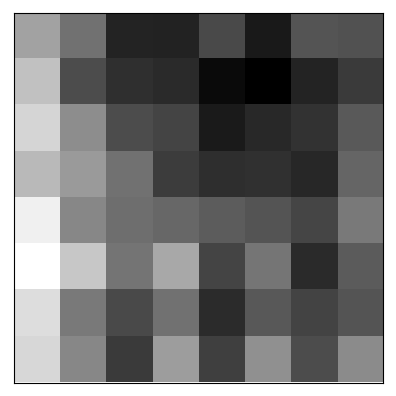
\includegraphics[scale=0.4]{figures/results/latent_image/beta_4_average_activation.png}
    \caption{$\beta=4$}
    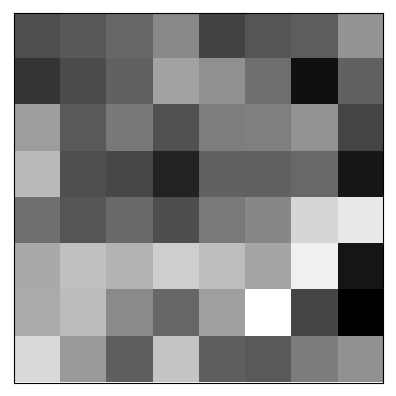
\includegraphics[scale=0.4]{figures/results/latent_image/beta_16_average_activation.png}
    \caption{$\beta=16$}
\end{multicols}
\caption{\textbf{Single latent filter architecture}. An average of the activations in the latent image over $10,000$ images from the test set for different values of $\beta$.}
\label{fig:latent_image_average_filters}
\end{figure*}




\clearpage
%
%
%
%
%
\section{Neuron-Level Redundancy Reduction}

\subsection{Results}
The multiple latent filter architecture, found in Table (\ref{tab:fully_convolutional_multiple_filter}), was trained for $10$ epochs with the neuron-level redundancy reduction loss function, and the validation, validation KL and validation reconstruction loss recorded. The results are shown in Figure (\ref{fig:indiscriminate_decoupling_graphs}). The multiple latent filter architecture with neuron-level redundancy reduction is clearly capable of achieving reasonable reconstruction and KL loss on unseen data, and achieves similar KL loss values as the single latent filter architecture, but considerably better reconstruction loss values.

Although the method reconstructs its input near perfectly, as shown in Figure (\ref{fig:indiscriminate_decoupling_originals_and_reconstructions}), the latent representations do not represent objects in the scene in an interpretable way. This is true also for the averaging of the latent filters over the $10,000$ test data points for all values of $\beta$. These results are shown in Figures (\ref{fig:indiscriminate_decoupling_originals_and_latent_filters}) and (\ref{fig:indiscriminate_decoupling_average_filters}) respectively.

Surprisingly, the decoded samples from the prior resemble the original scenes, shown in Figure (\ref{fig:indiscriminate_decoupling_prior_samples}). From these results, it's clear that the realism of these generated scenes improves with increasing $\beta$. As expected, the generative samples from the unknown distribution $\hat{p}(\vec{z})$ are more realistic. It's also clear that increasing $\beta$ encourages the samples from $\hat{p}(\vec{z})$ to stray further from the input, but in a statistically consistent way.

\subsection{Summary}

\begin{itemize}
\item The multiple latent filter architecture with neuron-level redundancy reduction is capable of near perfectly reconstructs of its input.
\item It also fails to learn interpretable latent representations of high-level concepts in the scene for all values of $\beta$.
\item However, it's capable of generating semi-realistic and statistically consistent samples. Varying $\beta$ has noticeable effects on the realism of the generative samples.
\end{itemize}



\begin{figure*}[h!]
\centering
\captionsetup{justification=centering}
    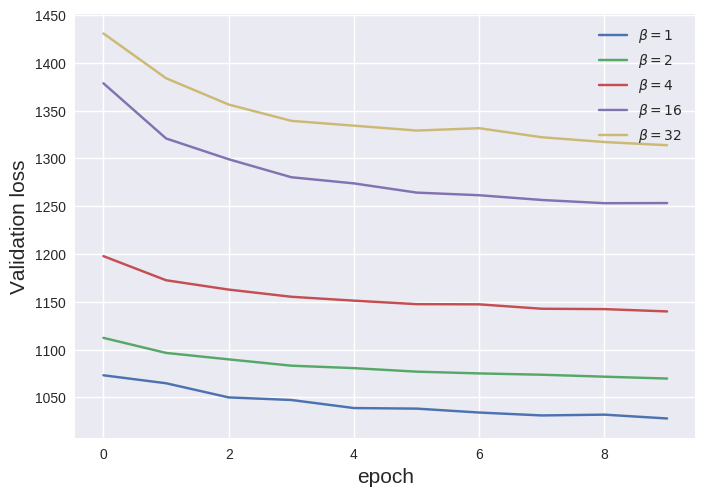
\includegraphics[scale=0.5]{figures/results/indiscriminate_decoupling/val_loss.png}
    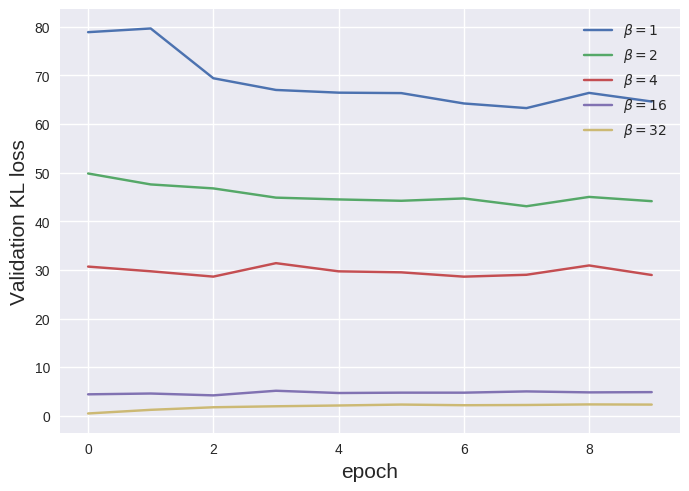
\includegraphics[scale=0.5]{figures/results/indiscriminate_decoupling/val_kl_loss.png}
    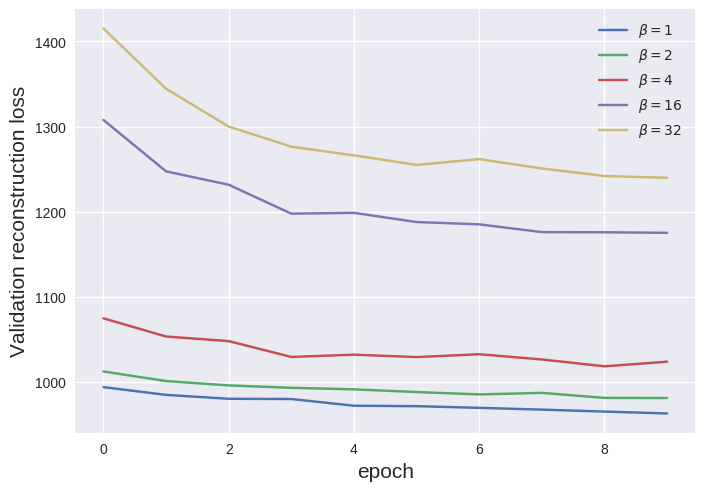
\includegraphics[scale=0.5]{figures/results/indiscriminate_decoupling/val_reconstruction_loss.png}
\caption{\textbf{Multiple latent filter archiecture with neuron-level redundancy reduction}. The validation, validation KL and validation reconstruction loss for the latent image architecture and different values of $\beta$.}
\label{fig:indiscriminate_decoupling_graphs}
\end{figure*}



\begin{figure*}[h!]
\centering
\captionsetup{justification=centering}
\begin{multicols}{4}
    \includegraphics[scale=0.4]{figures/results/indiscriminate_decoupling/beta_1_sample_0_original.png}
    \caption{Original}
    \includegraphics[scale=0.4]{figures/results/indiscriminate_decoupling/beta_1_sample_0_reconstructed.png}
    \caption{$\beta = 1$}    
    \includegraphics[scale=0.4]{figures/results/indiscriminate_decoupling/beta_4_sample_0_reconstructed.png}
    \caption{$\beta = 4$}
    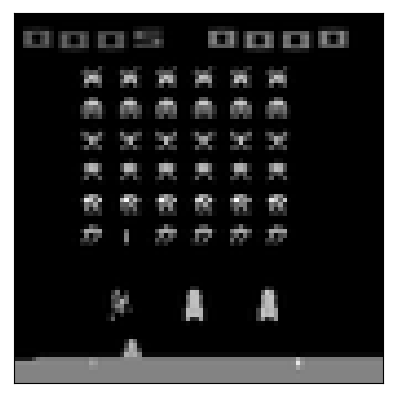
\includegraphics[scale=0.4]{figures/results/indiscriminate_decoupling/beta_32_sample_0_reconstructed.png}
    \caption{$\beta = 32$}
\end{multicols}
\begin{multicols}{4}
    \includegraphics[scale=0.4]{figures/results/indiscriminate_decoupling/beta_1_sample_2_original.png}
    \caption{Original}
    \includegraphics[scale=0.4]{figures/results/indiscriminate_decoupling/beta_1_sample_2_reconstructed.png}
    \caption{$\beta = 1$}    
    \includegraphics[scale=0.4]{figures/results/indiscriminate_decoupling/beta_4_sample_2_reconstructed.png}
    \caption{$\beta = 4$}
    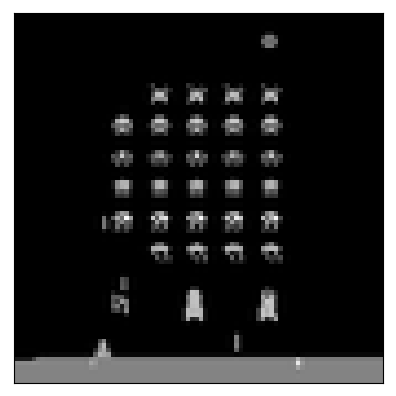
\includegraphics[scale=0.4]{figures/results/indiscriminate_decoupling/beta_32_sample_2_reconstructed.png}
    \caption{$\beta = 32$}
\end{multicols}
\begin{multicols}{4}
    \includegraphics[scale=0.4]{figures/results/indiscriminate_decoupling/beta_1_sample_3_original.png}
    \caption{Original}
    \includegraphics[scale=0.4]{figures/results/indiscriminate_decoupling/beta_1_sample_3_reconstructed.png}
    \caption{$\beta = 1$}
    \includegraphics[scale=0.4]{figures/results/indiscriminate_decoupling/beta_4_sample_3_reconstructed.png}
    \caption{$\beta = 4$}
    \includegraphics[scale=0.4]{figures/results/indiscriminate_decoupling/beta_32_sample_3_reconstructed.png}
    \caption{$\beta = 32$}
\end{multicols}
\caption{\textbf{Multiple latent filter architecture with neuron-level redundancy reduction}. A selection of Space Invader frames and their corresponding reconstructions for different values of $\beta$.}
\label{fig:indiscriminate_decoupling_originals_and_reconstructions}
\end{figure*}


\begin{figure*}[h!]
\centering
\captionsetup{justification=centering}
\begin{minipage}{0.4\textwidth}
\centering
\captionsetup{justification=centering}
\includegraphics[scale=0.4]{figures/results/indiscriminate_decoupling/beta_1_sample_3_original.png}
\caption{Original}
\end{minipage}
\begin{minipage}{0.55\textwidth}
\centering
\captionsetup{justification=centering}
\includegraphics[scale=0.42]{figures/results/indiscriminate_decoupling/beta_1_convolutional_layers_sample_3.png}
\caption{$\beta = 1$}
\includegraphics[scale=0.42]{figures/results/indiscriminate_decoupling/beta_4_convolutional_layers_sample_3.png}
\caption{$\beta = 4$}
\includegraphics[scale=0.42]{figures/results/indiscriminate_decoupling/beta_32_convolutional_layers_sample_3.png}
\caption{$\beta = 32$}
\end{minipage}
\caption{\textbf{Multiple latent filter architecture with neuron-level redundancy reduction}. A Space Invaders frame and the activations over its corresponding latent filters for different values of $\beta$.}
\label{fig:indiscriminate_decoupling_originals_and_latent_filters}
\end{figure*}


\begin{figure*}[h!]
\centering
\captionsetup{justification=centering}
\begin{multicols}{3}
    \includegraphics[scale=0.4]{figures/results/indiscriminate_decoupling/beta_1_prior_sample_2.png}
    \caption{$\beta=1$}
    \includegraphics[scale=0.4]{figures/results/indiscriminate_decoupling/beta_4_prior_sample_0.png}
    \caption{$\beta=4$}
    \includegraphics[scale=0.4]{figures/results/indiscriminate_decoupling/beta_32_prior_sample_3.png}
    \caption{$\beta=32$}
\end{multicols}
\caption{\textbf{Multiple latent filter architecture with neuron-level redundancy reduction}. The best of $10$ samples from the prior $p(\vec{z}) = \mathcal{N}(\vec{0}, \vec{I})$ for different values of $\beta$.}
\label{fig:indiscriminate_decoupling_prior_samples}
\end{figure*}


\begin{figure*}[h!]
\centering
\captionsetup{justification=centering}
\begin{multicols}{4}
    \includegraphics[scale=0.4]{figures/results/indiscriminate_decoupling/beta_1_posterior_sample_original.png}
    \caption{$\beta=1\quad$ (original)}
    \includegraphics[scale=0.4]{figures/results/indiscriminate_decoupling/beta_1_posterior_sample_10.png}
    \caption{$\beta=1\quad$ (19 steps)}
    \includegraphics[scale=0.4]{figures/results/indiscriminate_decoupling/beta_1_posterior_sample_26.png}
    \caption{$\beta=1\quad$ (26 steps)}
    \includegraphics[scale=0.4]{figures/results/indiscriminate_decoupling/beta_1_posterior_sample_60.png}
    \caption{$\beta=1\quad$ (60 steps)}
\end{multicols}

\begin{multicols}{4}
    \includegraphics[scale=0.4]{figures/results/indiscriminate_decoupling/beta_2_posterior_sample_original.png}
    \caption{$\beta=4\quad$ (original)}
    \includegraphics[scale=0.4]{figures/results/indiscriminate_decoupling/beta_4_posterior_sample_0.png}
    \caption{$\beta=4\quad$ (1 step)}
    \includegraphics[scale=0.4]{figures/results/indiscriminate_decoupling/beta_4_posterior_sample_7.png}
    \caption{$\beta=4\quad$ (7 steps)}
    \includegraphics[scale=0.4]{figures/results/indiscriminate_decoupling/beta_4_posterior_sample_98.png}
    \caption{$\beta=4\quad$ (98 steps)}
\end{multicols}

\begin{multicols}{4}
    \includegraphics[scale=0.4]{figures/results/indiscriminate_decoupling/beta_4_posterior_sample_original.png}
    \caption{$\beta=32\quad$ (original)}
    \includegraphics[scale=0.4]{figures/results/indiscriminate_decoupling/beta_32_posterior_sample_0.png}
    \caption{$\beta=32\quad$ (1 step)}
    \includegraphics[scale=0.4]{figures/results/indiscriminate_decoupling/beta_32_posterior_sample_16.png}
    \caption{$\beta=32\quad$ (15 steps)}
    \includegraphics[scale=0.4]{figures/results/indiscriminate_decoupling/beta_32_posterior_sample_49.png}
    \caption{$\beta=32\quad$ (48 steps)}
\end{multicols}

\caption{\textbf{Multiple latent filter architecture with neuron-level redundancy reduction}. A selection of Space Invader frames and the following samples from the unknown prior $\hat{p}(\vec{z})$ using MCMC for different values of $\beta$.}
\label{fig:indiscriminate_decoupling_posterior_samples}
\end{figure*}


\begin{figure*}[h!]
\centering
\captionsetup{justification=centering}

    \includegraphics[scale=0.3]{figures/results/indiscriminate_decoupling/beta_1_average_activation.png}
    \caption{$\beta=1$}
    \includegraphics[scale=0.3]{figures/results/indiscriminate_decoupling/beta_4_average_activation.png}
    \caption{$\beta=4$}
    \includegraphics[scale=0.3]{figures/results/indiscriminate_decoupling/beta_4_average_activation.png}
    \caption{$\beta=32$}

\caption{\textbf{Multiple latent filter architecture with neuron-level redundancy reduction}. An average of the activations in the latent image over $10,000$ images from the test set for different values of $\beta$.}
\label{fig:indiscriminate_decoupling_average_filters}
\end{figure*}






\clearpage
%
%
%
%
%
\section{Na{\"i}ve Filter-Level Redundancy Reduction}

\subsection{Results}
The multiple latent filter architecture, found in Table (\ref{tab:fully_convolutional_multiple_filter}), was trained for $10$ epochs with the na{\"i}ve filter-level redundancy reduction loss function, and the validation, validation KL and validation reconstruction loss recorded, which are shown in Figure (\ref{fig:naive_average_graphs}). As with previous methods, the image reconstructions are near perfect even for high $\beta$, as shown in Figure (\ref{fig:naive_average_originals_and_reconstructions}). 

Interestingly, in Figure (\ref{fig:naive_average_originals_and_latent_filters}), we see the beginnings of high-level objects in the latent filters! It's possible to make out the representation of the score bar for each value of $\beta$. We also see some very promising results on the average activations of the latent filters in Figure (\ref{fig:naive_average_average_filters}). The score bar and ground are recognised in at least one filter, with sometimes noticeable activations on the barriers. The value of $\beta$ does not have a noticeable influence on the latent filters. 

Further, we see that the samples from the prior $p(\vec{z})$ are far from resembling the original scene, but samples from the unknown distribution $\hat{p}(\vec{z})$ are very realistic for high $\beta$! We expect poor samples from the prior as we pressure $\bar{\vec{\mu}}$ and $\bar{\vec{\sigma}}$ to be close to $p(\vec{z})$, not $\vec{\mu}$ and $\vec{\sigma}$ as before.

\subsection{Summary}
\begin{itemize}
\item As with the previous methods, the na{\"i}ve filter-level redundancy reduction method near perfectly reconstructs its inputs irrespective of the value of $\beta$.
\item The method achieves the first signs of latent filter representations of high-level objects in the scene. This is especially obvious in the average activations of latent filters, where the score, floor and barriers are clearly recognised.
\item However, the generative power of this method is quite strong. Samples from the unknown distribution $\hat{p}(\vec{z})$ resemble the original scene after a threshold value of $\beta$.
\item We therefore have a method that learns persistent high-level features and may generate realistic novel samples.
\end{itemize}


\begin{figure*}[h!]
\centering
\captionsetup{justification=centering}
    \includegraphics[scale=0.5]{figures/results/naive_average/val_loss.png}
    \includegraphics[scale=0.5]{figures/results/naive_average/val_kl_loss.png}
    \includegraphics[scale=0.5]{figures/results/naive_average/val_reconstruction_loss.png}
\caption{\textbf{Multiple latent filter architecture with na{\"i}ve filter-level redundancy reduction}. The validation, validation KL and validation reconstruction loss for the latent image architecture and different values of $\beta$. The validation reconstruction loss for $\beta = 16, 32$ were $\sim 950$, and are therefore excluded in two plots for readability.}
\label{fig:naive_average_graphs}
\end{figure*}


\begin{figure*}[h!]
\centering
\captionsetup{justification=centering}
\begin{multicols}{4}
    \includegraphics[scale=0.4]{figures/results/naive_average/beta_1_sample_0_original.png}
    \caption{Original}
    \includegraphics[scale=0.4]{figures/results/naive_average/beta_1_sample_0_reconstructed.png}
    \caption{$\beta = 1$}    
    \includegraphics[scale=0.4]{figures/results/naive_average/beta_2_sample_0_reconstructed.png}
    \caption{$\beta = 2$}
    \includegraphics[scale=0.4]{figures/results/naive_average/beta_32_sample_0_reconstructed.png}
    \caption{$\beta = 32$}
\end{multicols}
\begin{multicols}{4}
    \includegraphics[scale=0.4]{figures/results/naive_average/beta_1_sample_2_original.png}
    \caption{Original}
    \includegraphics[scale=0.4]{figures/results/naive_average/beta_1_sample_2_reconstructed.png}
    \caption{$\beta = 1$}    
    \includegraphics[scale=0.4]{figures/results/naive_average/beta_2_sample_2_reconstructed.png}
    \caption{$\beta = 2$}
    \includegraphics[scale=0.4]{figures/results/naive_average/beta_4_sample_2_reconstructed.png}
    \caption{$\beta = 4$}
\end{multicols}
\begin{multicols}{4}
    \includegraphics[scale=0.4]{figures/results/naive_average/beta_1_sample_3_original.png}
    \caption{Original}
    \includegraphics[scale=0.4]{figures/results/naive_average/beta_1_sample_3_reconstructed.png}
    \caption{$\beta = 1$}
    \includegraphics[scale=0.4]{figures/results/naive_average/beta_2_sample_3_reconstructed.png}
    \caption{$\beta = 2$}
    \includegraphics[scale=0.4]{figures/results/naive_average/beta_4_sample_3_reconstructed.png}
    \caption{$\beta = 4$}
\end{multicols}
\caption{\textbf{Multiple latent filter architecture with na{\"i}ve filter-level redundancy reduction}. A selection of Space Invader frames and their corresponding reconstructions for different values of $\beta$.}
\label{fig:naive_average_originals_and_reconstructions}
\end{figure*}



\begin{figure*}[h!]
\centering
\captionsetup{justification=centering}
\begin{minipage}{0.4\textwidth}
\centering
\captionsetup{justification=centering}
\includegraphics[scale=0.4]{figures/results/naive_average/beta_1_sample_3_original.png}
\caption{Original}
\end{minipage}
\begin{minipage}{0.55\textwidth}
\centering
\captionsetup{justification=centering}
\includegraphics[scale=0.42]{figures/results/naive_average/beta_1_convolutional_layers_sample_3.png}
\caption{$\beta = 1$}
\includegraphics[scale=0.42]{figures/results/naive_average/beta_4_convolutional_layers_sample_3.png}
\caption{$\beta = 4$}
\includegraphics[scale=0.42]{figures/results/naive_average/beta_32_convolutional_layers_sample_3.png}
\caption{$\beta = 32$}
\end{minipage}
\caption{\textbf{Multiple latent filter architecture with na{\"i}ve filter-level redundancy reduction}. A Space Invaders frame and the activations over its corresponding latent filters for different values of $\beta$.}
\label{fig:naive_average_originals_and_latent_filters}
\end{figure*}



\begin{figure*}[h!]
\centering
\captionsetup{justification=centering}
\begin{multicols}{3}
    \includegraphics[scale=0.4]{figures/results/naive_average/beta_1_prior_sample_2.png}
    \caption{$\beta=1$}
    \includegraphics[scale=0.4]{figures/results/naive_average/beta_4_prior_sample_0.png}
    \caption{$\beta=4$}
    \includegraphics[scale=0.4]{figures/results/naive_average/beta_32_prior_sample_3.png}
    \caption{$\beta=32$}
\end{multicols}
\caption{\textbf{Multiple latent filter architecture with na{\"i}ve filter-level redundancy reduction}. The best of $10$ samples from the prior $p(\vec{z}) = \mathcal{N}(\vec{0}, \vec{I})$ for different values of $\beta$.}
\label{fig:naive_average_decoupling_prior_samples}
\end{figure*}


\begin{figure*}[h!]
\centering
\captionsetup{justification=centering}
\begin{multicols}{4}
    \includegraphics[scale=0.4]{figures/results/naive_average/beta_1_posterior_sample_original.png}
    \caption{$\beta=1\quad$ (original)}
    \includegraphics[scale=0.4]{figures/results/naive_average/beta_1_posterior_sample_0.png}
    \caption{$\beta=1\quad$ (1 step)}
    \includegraphics[scale=0.4]{figures/results/naive_average/beta_1_posterior_sample_5.png}
    \caption{$\beta=1\quad$ (5 steps)}
    \includegraphics[scale=0.4]{figures/results/naive_average/beta_1_posterior_sample_10.png}
    \caption{$\beta=1\quad$ (10 steps)}
\end{multicols}

\begin{multicols}{4}
    \includegraphics[scale=0.4]{figures/results/naive_average/beta_2_posterior_sample_original.png}
    \caption{$\beta=4\quad$ (original)}
    \includegraphics[scale=0.4]{figures/results/naive_average/beta_4_posterior_sample_0.png}
    \caption{$\beta=4\quad$ (1 step)}
    \includegraphics[scale=0.4]{figures/results/naive_average/beta_4_posterior_sample_5.png}
    \caption{$\beta=4\quad$ (5 steps)}
    \includegraphics[scale=0.4]{figures/results/naive_average/beta_4_posterior_sample_10.png}
    \caption{$\beta=4\quad$ (10 steps)}
\end{multicols}

\begin{multicols}{4}
    \includegraphics[scale=0.4]{figures/results/naive_average/beta_4_posterior_sample_original.png}
    \caption{$\beta=32\quad$ (original)}
    \includegraphics[scale=0.4]{figures/results/naive_average/beta_32_posterior_sample_0.png}
    \caption{$\beta=32\quad$ (1 step)}
    \includegraphics[scale=0.4]{figures/results/naive_average/beta_32_posterior_sample_5.png}
    \caption{$\beta=32\quad$ (5 steps)}
    \includegraphics[scale=0.4]{figures/results/naive_average/beta_32_posterior_sample_10.png}
    \caption{$\beta=32\quad$ (10 steps)}
\end{multicols}

\caption{\textbf{Multiple latent filter architecture with na{\"i}ve filter-level redundancy reduction}. A selection of Space Invader frames and the following samples from the unknown prior $\hat{p}(\vec{z})$ using MCMC for different values of $\beta$.}
\label{fig:naive_average_originals_posterior_samples}
\end{figure*}


\begin{figure*}[h!]
\centering
\captionsetup{justification=centering}

    \includegraphics[scale=0.3]{figures/results/naive_average/beta_1_average_activation.png}
    \caption{$\beta=1$}
    \includegraphics[scale=0.3]{figures/results/naive_average/beta_4_average_activation.png}
    \caption{$\beta=4$}
    \includegraphics[scale=0.42]{figures/results/naive_average/beta_32_average_activation.png}
    \caption{$\beta=32$}

\caption{\textbf{Multiple latent filter architecture with na{\"i}ve filter-level redundancy reduction}. An average of the activations in the latent image over $10,000$ images from the test set for different values of $\beta$.}
\label{fig:naive_average_average_filters}
\end{figure*}




\clearpage
%
%
%
%
%
\section{Weighted Filter-Level Redundancy Reduction}

\subsection{Results}
The multiple latent filter architecture, found in Table (\ref{tab:fully_convolutional_multiple_filter}), was trained for $10$ epochs with the na{\"i}ve filter-level redundancy reduction loss function, and the validation, validation KL and validation reconstruction loss recorded, which are shown in Figure (\ref{fig:weighted_average_graphs}). Despite the large weight on the KL loss term, the image reconstructions are near perfect for all $\beta$, as shown in Figure (\ref{fig:weighted_average_originals_and_reconstructions}). 

High-level objects are clearly represented in the latent filters, particularly for $\beta = 4$. The barriers and score are again clearly identified in the latent filters. This does not seem to be the case with $\beta = 32$, which suggests there is an optimal value of $\beta$. Further, the average activations of the latent filters in Figure (\ref{fig:weighted_average_average_filters}) show that, on average, $\beta = 4$ and $\beta = 32$ both detect persistent high-level objects in the scene.

When comparing the input to the corresponding latent filters, we find an interesting result. We can easily spot the barriers and score for $\beta=4$, but not so for $\beta = 32$, as shown in Figure (\ref{fig:weighted_average_originals_and_latent_filters}). Further, the samples from the unknown distribution $\hat{p}(\vec{z})$ are much more interesting for $\beta = 4$ than $\beta = 32$. For $\beta = 32$, the samples do not differ very much from its input, whereas samples for $\beta = 4$ differ widely (bullets disappear and scores change), but in a realistic consistent way. These results are shown in Figure (\ref{fig:weighted_average_posterior_samples}).

\subsection{Summary}

\begin{itemize}
\item The method is capable of near perfectly reconstructing the original image, despite having a large multiplicative factor on the KL loss term.
\item Latent representations of persistent high-level objects in the scene are clear for some $\beta$.
\item Further, values of $\beta$ also have a noticeable effect on the generated samples from the unknown distribution $\hat{p}(\vec{z})$.
\end{itemize}



\begin{figure*}[h!]
\centering
\captionsetup{justification=centering}
    \includegraphics[scale=0.5]{figures/results/weighted_average/val_loss.png}
    \includegraphics[scale=0.5]{figures/results/weighted_average/val_kl_loss.png}
    \includegraphics[scale=0.5]{figures/results/weighted_average/val_reconstruction_loss.png}
\caption{\textbf{Multiple latent filter architecture with weighted filter-level redundancy reduction}. The validation, validation KL and validation reconstruction loss for the latent image architecture and different values of $\beta$.}
\label{fig:weighted_average_graphs}
\end{figure*}




\begin{figure*}[h!]
\centering
\captionsetup{justification=centering}
\begin{multicols}{4}
    \includegraphics[scale=0.4]{figures/results/weighted_average/beta_1_sample_0_original.png}
    \caption{Original}
    \includegraphics[scale=0.4]{figures/results/weighted_average/beta_1_sample_0_reconstructed.png}
    \caption{$\beta = 1$}    
    \includegraphics[scale=0.4]{figures/results/weighted_average/beta_4_sample_0_reconstructed.png}
    \caption{$\beta = 4$}
    \includegraphics[scale=0.4]{figures/results/weighted_average/beta_32_sample_0_reconstructed.png}
    \caption{$\beta = 32$}
\end{multicols}
\begin{multicols}{4}
    \includegraphics[scale=0.4]{figures/results/weighted_average/beta_1_sample_2_original.png}
    \caption{Original}
    \includegraphics[scale=0.4]{figures/results/weighted_average/beta_1_sample_2_reconstructed.png}
    \caption{$\beta = 1$}    
    \includegraphics[scale=0.4]{figures/results/weighted_average/beta_4_sample_2_reconstructed.png}
    \caption{$\beta = 4$}
    \includegraphics[scale=0.4]{figures/results/weighted_average/beta_32_sample_2_reconstructed.png}
    \caption{$\beta = 32$}
\end{multicols}
\begin{multicols}{4}
    \includegraphics[scale=0.4]{figures/results/weighted_average/beta_1_sample_3_original.png}
    \caption{Original}
    \includegraphics[scale=0.4]{figures/results/weighted_average/beta_1_sample_3_reconstructed.png}
    \caption{$\beta = 1$}
    \includegraphics[scale=0.4]{figures/results/weighted_average/beta_4_sample_3_reconstructed.png}
    \caption{$\beta = 4$}
    \includegraphics[scale=0.4]{figures/results/weighted_average/beta_32_sample_3_reconstructed.png}
    \caption{$\beta = 32$}
\end{multicols}
\caption{\textbf{Multiple latent filter architecture with weighted filter-level redundancy reduction}. A selection of Space Invader frames and their corresponding reconstructions for different values of $\beta$.}
\label{fig:weighted_average_originals_and_reconstructions}
\end{figure*}




\begin{figure*}[h!]
\centering
\captionsetup{justification=centering}
\begin{minipage}{0.4\textwidth}
\centering
\captionsetup{justification=centering}
\includegraphics[scale=0.4]{figures/results/weighted_average/beta_1_sample_3_original.png}
\caption{Original}
\end{minipage}
\begin{minipage}{0.55\textwidth}
\centering
\captionsetup{justification=centering}
\includegraphics[scale=0.42]{figures/results/weighted_average/beta_1_convolutional_layers_sample_3.png}
\caption{$\beta = 1$}
\includegraphics[scale=0.42]{figures/results/weighted_average/beta_4_convolutional_layers_sample_3.png}
\caption{$\beta = 4$}
\includegraphics[scale=0.42]{figures/results/weighted_average/beta_32_convolutional_layers_sample_3.png}
\caption{$\beta = 32$}
\end{minipage}
\caption{\textbf{Multiple latent filter architecture with weighted filter-level redundancy reduction}. A Space Invaders frame and the activations over its corresponding latent filters for different values of $\beta$.}
\label{fig:weighted_average_originals_and_latent_filters}
\end{figure*}

\begin{figure*}[h!]
\centering
\captionsetup{justification=centering}
\begin{multicols}{4}
    \includegraphics[scale=0.4]{figures/results/weighted_average/beta_1_posterior_sample_original.png}
    \caption{$\beta=1\quad$ (original)}
    \includegraphics[scale=0.4]{figures/results/weighted_average/beta_1_posterior_sample_18.png}
    \caption{$\beta=1\quad$ (18 steps)}
    \includegraphics[scale=0.4]{figures/results/weighted_average/beta_1_posterior_sample_26.png}
    \caption{$\beta=1\quad$ (26 steps)}
    \includegraphics[scale=0.4]{figures/results/weighted_average/beta_1_posterior_sample_39.png}
    \caption{$\beta=1\quad$ (39 steps)}
\end{multicols}

\begin{multicols}{4}
    \includegraphics[scale=0.4]{figures/results/weighted_average/beta_4_posterior_sample_original.png}
    \caption{$\beta=4\quad$ (original)}
    \includegraphics[scale=0.4]{figures/results/weighted_average/beta_4_posterior_sample_0.png}
    \caption{$\beta=4\quad$ (1 step)}
    \includegraphics[scale=0.4]{figures/results/weighted_average/beta_4_posterior_sample_7.png}
    \caption{$\beta=4\quad$ (5 steps)}
    \includegraphics[scale=0.4]{figures/results/weighted_average/beta_4_posterior_sample_47.png}
    \caption{$\beta=4\quad$ (40 steps)}
\end{multicols}

\begin{multicols}{4}
    \includegraphics[scale=0.4]{figures/results/weighted_average/beta_32_posterior_sample_original.png}
    \caption{$\beta=32\quad$ (original)}
    \includegraphics[scale=0.4]{figures/results/weighted_average/beta_32_posterior_sample_1.png}
    \caption{$\beta=32\quad$ (1 step)}
    \includegraphics[scale=0.4]{figures/results/weighted_average/beta_32_posterior_sample_47.png}
    \caption{$\beta=32\quad$ (47 steps)}
    \includegraphics[scale=0.4]{figures/results/weighted_average/beta_32_posterior_sample_62.png}
    \caption{$\beta=32\quad$ (62 steps)}
\end{multicols}

\caption{\textbf{Multiple latent filter architecture with weighted filter-level redundancy reduction}. A selection of Space Invader frames and the following samples from the unknown prior $\hat{p}(\vec{z})$ using MCMC for different values of $\beta$.}
\label{fig:weighted_average_posterior_samples}
\end{figure*}



\begin{figure*}[h!]
\centering
\captionsetup{justification=centering}

    \includegraphics[scale=0.42]{figures/results/weighted_average/beta_1_average_activation.png}
    \caption{$\beta=1$}
    \includegraphics[scale=0.42]{figures/results/weighted_average/beta_2_average_activation.png}
    \caption{$\beta=2$}
    \includegraphics[scale=0.42]{figures/results/weighted_average/beta_4_average_activation.png}
    \caption{$\beta=4$}

\caption{\textbf{Multiple latent filter architecture with weighted filter-level redundancy reduction}. An average of the activations in the latent image over $10,000$ images from the test set for different values of $\beta$.}
\label{fig:weighted_average_average_filters}
\end{figure*}




\clearpage
%
%
%
%
%
\section{Separating Colour Spaces}

\subsection{Results}
The multiple latent filter RGB architecture, found in Table (\ref{tab:fully_convolutional_multiple_filter_rgb}), was trained for $15$ epochs, and the validation, validation KL and validation reconstruction loss recorded.

The reconstructions for RGB images were poor compared to their greyscale equivalents. For example, in Figure (\ref{fig:colour_separated_originals_and_reconstructions}), $\beta = 2$ fails to reconstruct individual space invaders, and $\beta = 4$ fails to reconstruct entire columns.

Figure (\ref{fig:colour_separated_originals_and_latent_filters}) shows that the latent filters fail to meaningfully learn an interpretable representation of the original input. However, the average activations have detected the persistent score bar at the top of the frame, shown in Figure (\ref{fig:colour_separated_average_filters}). The value of $\beta$ appears to have no effect on the latent filters.

Samples from the unknown distribution, $\hat{p}(\vec{z})$ shown in Figure (\ref{fig:colour_separated_posterior_samples}), are reasonable for a small number of steps of MCMC. The generative samples quickly begin to look unrealistic with more than $40$ steps. Here the value of $\beta$ seems to encourage the generated images more realistic.

The poor results for this method are likely due to the increase in dimensionality of the input. If left to train for a sufficiently long time, we suspect this would improve the model.

\subsection{Summary}

\begin{itemize}
\item The increase in dimensionality of the input requires a non-trivial amount of more time training. It is likely this method will do at least as well as with greyscale images.
\item For this particular test, the reconstructions were the worst out of every method
\item The method struggled to learn interpretable latent representations
\item Show reconstructions and convolutional layers of each
\end{itemize}




\begin{figure*}[h!]
\centering
\captionsetup{justification=centering}
\begin{multicols}{4}
    \includegraphics[scale=0.4]{figures/results/colour_separated/beta_1_sample_0_original.png}
    \caption{Original}
    \includegraphics[scale=0.4]{figures/results/colour_separated/beta_1_sample_0_reconstructed.png}
    \caption{$\beta = 1$}    
    \includegraphics[scale=0.4]{figures/results/colour_separated/beta_2_sample_0_reconstructed.png}
    \caption{$\beta = 2$}
    \includegraphics[scale=0.4]{figures/results/colour_separated/beta_4_sample_0_reconstructed.png}
    \caption{$\beta = 4$}
\end{multicols}
\begin{multicols}{4}
    \includegraphics[scale=0.4]{figures/results/colour_separated/beta_1_sample_2_original.png}
    \caption{Original}
    \includegraphics[scale=0.4]{figures/results/colour_separated/beta_1_sample_2_reconstructed.png}
    \caption{$\beta = 1$}    
    \includegraphics[scale=0.4]{figures/results/colour_separated/beta_2_sample_2_reconstructed.png}
    \caption{$\beta = 2$}
    \includegraphics[scale=0.4]{figures/results/colour_separated/beta_4_sample_2_reconstructed.png}
    \caption{$\beta = 4$}
\end{multicols}
\begin{multicols}{4}
    \includegraphics[scale=0.4]{figures/results/colour_separated/beta_1_sample_3_original.png}
    \caption{Original}
    \includegraphics[scale=0.4]{figures/results/colour_separated/beta_1_sample_3_reconstructed.png}
    \caption{$\beta = 1$}    
    \includegraphics[scale=0.4]{figures/results/colour_separated/beta_2_sample_3_reconstructed.png}
    \caption{$\beta = 2$}
    \includegraphics[scale=0.4]{figures/results/colour_separated/beta_4_sample_3_reconstructed.png}
    \caption{$\beta = 4$}
\end{multicols}
\caption{\textbf{Multiple latent filter architecture for RGB with weighted filter-level redundancy reduction}. A selection of Space Invader frames and their corresponding reconstructions for different values of $\beta$.}
\label{fig:colour_separated_originals_and_reconstructions}
\end{figure*}



\begin{figure*}[h!]
\centering
\captionsetup{justification=centering}
\begin{minipage}{0.4\textwidth}
\centering
\captionsetup{justification=centering}
\includegraphics[scale=0.4]{figures/results/colour_separated/beta_1_sample_3_original.png}
\caption{Original}
\end{minipage}
\begin{minipage}{0.55\textwidth}
\centering
\captionsetup{justification=centering}
\includegraphics[scale=0.42]{figures/results/colour_separated/beta_1_convolutional_layers_sample_3.png}
\caption{$\beta = 1$}
\includegraphics[scale=0.42]{figures/results/colour_separated/beta_2_convolutional_layers_sample_3.png}
\caption{$\beta = 2$}
\includegraphics[scale=0.42]{figures/results/colour_separated/beta_4_convolutional_layers_sample_3.png}
\caption{$\beta = 4$}
\end{minipage}
\caption{\textbf{Multiple latent filter architecture for RGB with weighted filter-level redundancy reduction}. A Space Invaders frame and the activations over its corresponding latent filters for different values of $\beta$.}
\label{fig:colour_separated_originals_and_latent_filters}
\end{figure*}






\begin{figure*}[h!]
\centering
\captionsetup{justification=centering}
\begin{multicols}{4}
    \includegraphics[scale=0.4]{figures/results/colour_separated/beta_1_posterior_sample_original.png}
    \caption{$\beta=1\quad$ (original)}
    \includegraphics[scale=0.4]{figures/results/colour_separated/beta_1_posterior_sample_7.png}
    \caption{$\beta=1\quad$ (7 steps)}
    \includegraphics[scale=0.4]{figures/results/colour_separated/beta_1_posterior_sample_13.png}
    \caption{$\beta=1\quad$ (17 steps)}
    \includegraphics[scale=0.4]{figures/results/colour_separated/beta_1_posterior_sample_18.png}
    \caption{$\beta=1\quad$ (18 steps)}
\end{multicols}

\begin{multicols}{4}
    \includegraphics[scale=0.4]{figures/results/colour_separated/beta_2_posterior_sample_original.png}
    \caption{$\beta=2\quad$ (original)}
    \includegraphics[scale=0.4]{figures/results/colour_separated/beta_2_posterior_sample_10.png}
    \caption{$\beta=2\quad$ (10 steps)}
    \includegraphics[scale=0.4]{figures/results/colour_separated/beta_2_posterior_sample_17.png}
    \caption{$\beta=2\quad$ (17 steps)}
    \includegraphics[scale=0.4]{figures/results/colour_separated/beta_2_posterior_sample_31.png}
    \caption{$\beta=2\quad$ (31 steps)}
\end{multicols}

\begin{multicols}{4}
    \includegraphics[scale=0.4]{figures/results/colour_separated/beta_4_posterior_sample_original.png}
    \caption{$\beta=4\quad$ (original)}
    \includegraphics[scale=0.4]{figures/results/colour_separated/beta_4_posterior_sample_1.png}
    \caption{$\beta=4\quad$ (1 step)}
    \includegraphics[scale=0.4]{figures/results/colour_separated/beta_4_posterior_sample_4.png}
    \caption{$\beta=4\quad$ (3 steps)}
    \includegraphics[scale=0.4]{figures/results/colour_separated/beta_4_posterior_sample_20.png}
    \caption{$\beta=4\quad$ (20 steps)}
\end{multicols}

\caption{\textbf{Multiple latent filter architecture for RGB with weighted filter-level redundancy reduction}. A selection of Space Invader frames and the following samples from the unknown prior $\hat{p}(\vec{z})$ using MCMC for different values of $\beta$.}
\label{fig:colour_separated_posterior_samples}
\end{figure*}


\begin{figure*}[h!]
\centering
\captionsetup{justification=centering}

    \includegraphics[scale=0.42]{figures/results/colour_separated/beta_1_average_activation.png}
    \caption{$\beta=1$}
    \includegraphics[scale=0.42]{figures/results/colour_separated/beta_2_average_activation.png}
    \caption{$\beta=2$}
    \includegraphics[scale=0.42]{figures/results/colour_separated/beta_4_average_activation.png}
    \caption{$\beta=4$}

\caption{\textbf{Multiple latent filter architecture for RGB with weighted filter-level redundancy reduction}. An average of the activations in the latent image over $10,000$ images from the test set for different values of $\beta$.}
\label{fig:colour_separated_average_filters}
\end{figure*}